\documentclass[13pt]{article}
\usepackage[english]{babel}
\usepackage{natbib}
\usepackage{url}
\usepackage[utf8x]{inputenc}
\usepackage{amsmath}
\usepackage{graphicx}
\graphicspath{{images/}}
\usepackage{parskip}
\usepackage{fancyhdr}
\usepackage{vmargin}
\usepackage{minted}
\setmarginsrb{3 cm}{2.5 cm}{3 cm}{2.5 cm}{1 cm}{1.5 cm}{1 cm}{1.5 cm}


							


\makeatletter
\let\thetitle\@title

\let\thedate\@date
\makeatother

\pagestyle{fancy}
\fancyhf{}
\rhead{\theauthor}
\lhead{\thetitle}
\cfoot{\thepage}

\begin{document}

%%%%%%%%%%%%%%%%%%%%%%%%%%%%%%%%%%%%%%%%%%%%%%%%%%%%%%%%%%%%%%%%%%%%%%%%%%%%%%%%%%%%%%%%%

\begin{titlepage}
	\centering
    \vspace*{0.5 cm}
    % \includegraphics[scale = 0.35]{City-Logo.jpg}\\[1.0 cm]	% University Logo
    \textsc{\LARGE Indian Institute of Technology}\\[2.0 cm]
    \textsc{\lARGE COMPUTER SCIENCE AND ENGINEERING}\\[0.2 cm]
    \textsc{\lARGE Software Lab}\\[0.2 cm]
	\textsc{\Large CS699}\\[0.5 cm]				% Course Code
	\textsc{\large QMark\\Question Bank}\\[0.2 cm]
	\rule{\linewidth}{0.2 mm} \\[0.4 cm]
	{ \huge \bfseries \thetitle}\\
	
	
	\begin{minipage}{0.4\textwidth}
		
			\begin{flushright} 
			Sourab Jha 19305R003\linebreak
			Devesh Ratna Singh 193050024\linebreak
			Zahid Wakeel 193050076\linebreak
			
		\end{flushright}
	\end{minipage}\\[2 cm]
	

 
	\vfill
	
\end{titlepage}

\tableofcontents
\pagebreak


\section{Introduction}

\justifying
QMark is an application for all of your academic needs at one place. Here you can store and access all of the questions and question papers added to our database so far, properly tagged with our multi-topic hierarchical topic. \par The aim of this application is to provide a simple, intuitive, and useful interface for setting up question papers for practice and exam alike, such that the instructors has to spend minimal time in browsing through old archives and the web to set a paper. Papers can be set using old questions papers spanning across the database, or using new questions created in the application itself. Students can check their understanding of certain topics by attempting questions from these topics.

\newpage
\section{Motivation}
Tests are conducted to assess student's knowledge in a subject, grading them, to give admission to higher education, placements, scholarships, etc. Hence, a question paper must be set in a way that can measure the change in the level of students' knowledge in a particular subject. Therefore, a good amount of care and caution is necessary for setting question papers. The types of question papers differ with the objective of the examination.\par

The process of setting a new question paper for an examination could be cumbersome and tedious when one has to dig through old archives and comply with the guidelines at the same time. A centralized, one-size-fits-all approach to collaborative setting of papers either do not exist or are not intuitive enough to be popular.\par

One has to keep in mind the difficulty level of each question, check questions against previous papers, and still cover the various topics or skills that need to be assessed. This mental overhead hampers setting up quality papers.\par

An aspirant usually covers her syllabi in a topic-wise fashion, wherein applications of multiple topics or skills come in later than application of individual topics. However, question banks usually do not account for this distinction between topics covered and not covered. Thus, a practice session tailored for individual needs is not trivially set up.\par


\newpage
\begin{figure}[H]
    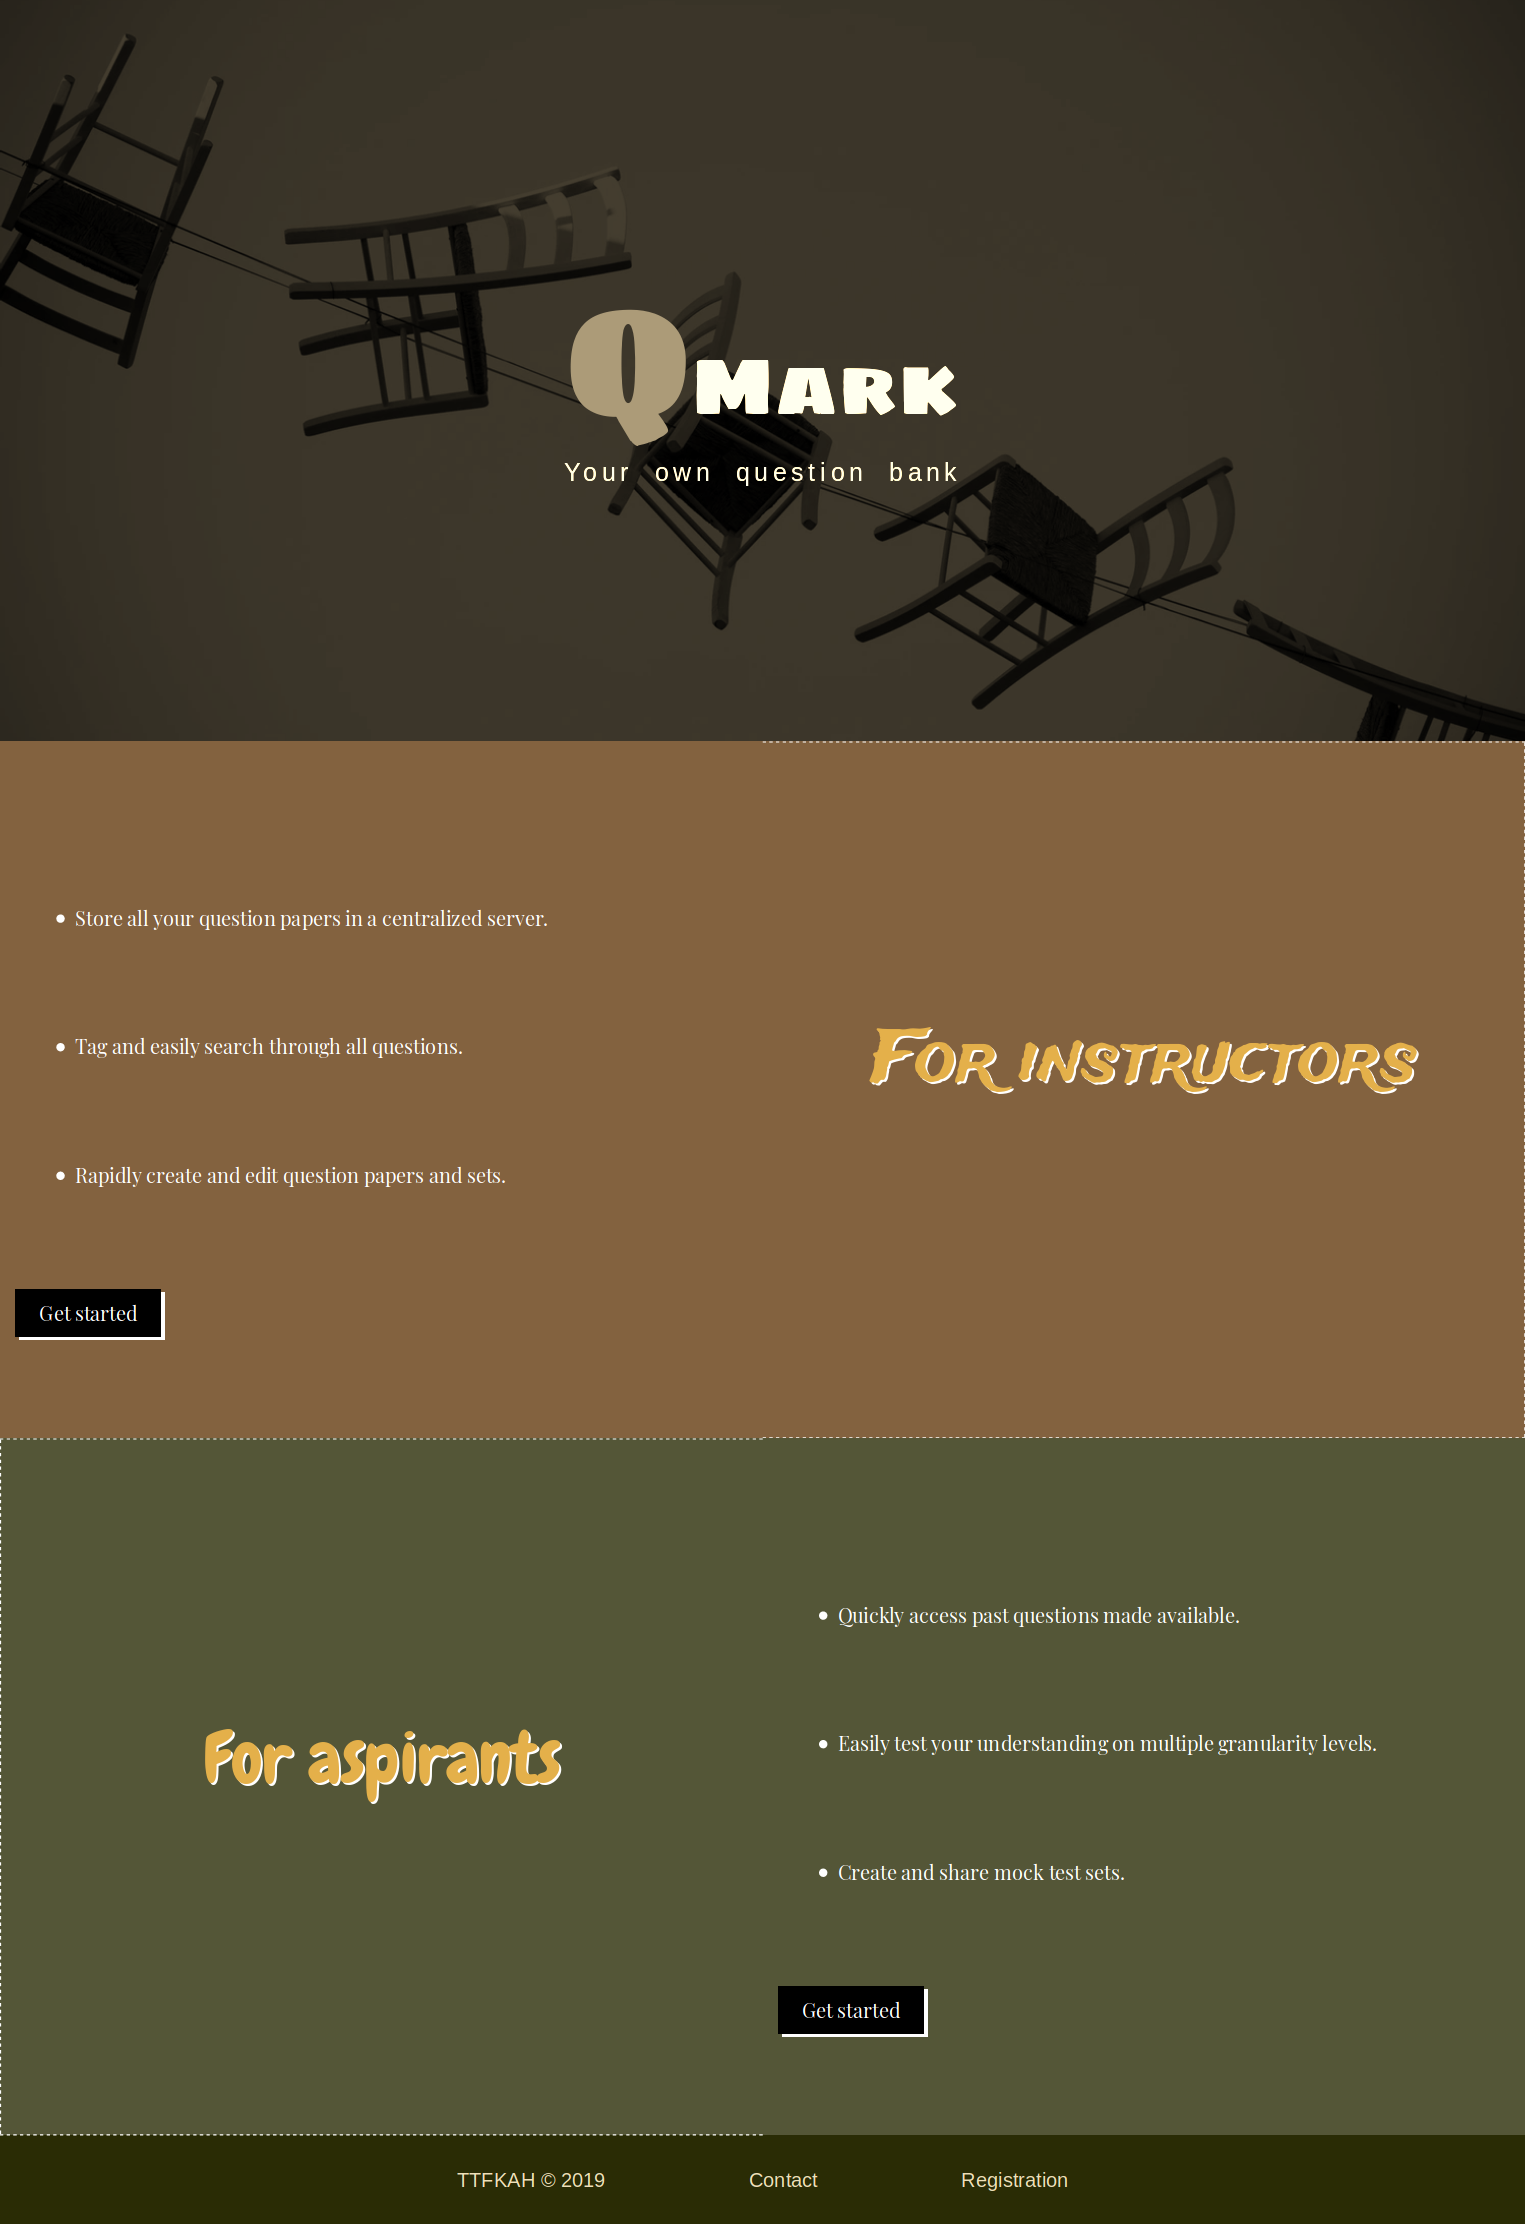
\includegraphics[width=\textwidth,height=\textheight,keepaspectratio]{home.png}
    
    \caption{Approximate Landing Page of QMark on desktop, across 3 vertical screens}
    \label{fig:home}
\end{figure}
\section{Installation}

Installation on a Linux distribution is recommended, and we only cover installation on Ubuntu, although one can easily follow the equivalent of these steps on Windows, or other *nix distributions for the same results.\par
Availability of python3.x on the system is also assumed.
\begin{minted}[
% bgcolor=LightGray
]{bash}
    # Create a virtualenv
    sudo apt install virtualenv

    # Clone the repository from github
    git clone git@github.com:hundredrab/QuestionBank.git
    # Alternatively:
    # git clone https://github.com/hundredrab/QuestionBank
    
    cd QuestionBank/source
    
    # Create and source a new virtualenv
    virtualenv -p python3 env
    source env/bin/activate
    
    # Set up the environment
    pip install -r requirements.txt
    
    # Apply the migrations and start the development server
    python manage.py migrate
    python manage.py createsuperuser
    python manage.py runserver
\end{minted}

The above code will install all the requirements, the major ones being Django, django-rest-framework, and fitz.
Once these steps are complete, the development server should be running on \texttt{http://localhost:8000/}, somewhat as shown in Fig \ref{fig:home}.\par

For development, it will also be necessary to install \texttt{sass} using the following command:\par
\begin{minted}{bash}
npm install -g sass
\end{minted}
\newpage

\section{Overview}
The webapp uses Django and contains two major apps, \texttt{questions} and \texttt{accounts}. The latter is only responsible for account and user related views and logic.\par

The \texttt{question} app consists of the rest of the logic. The major components of this app are:\\\\
\par
% \begin{itemize}
    \subsection{Tag}
    This model stores information related to tags. Each node, except the \texttt{root} node has a \texttt{parent} associated with it. The immediate children of the root node are major subject areas such as Science, Humanities, etc.\\
    
    \subsection{QuestionPaper}

    This relation is used for storing the question papers uploaded by the user.\par
    On upload, the question paper is parsed using fitz and the raw text thus extracted is stored with the question paper. The uploader can go through the raw text and select certain questions from it.\\
    
    \subsection{Question}

    This stores information related to a question, such as the question \texttt{text}, \texttt{tags} related to it, it's \texttt{owner}, and also it's \texttt{difficulty}, which an integer, which is an indicator of how much marks should be awarded for the given question.\\

    \subsection{QuestionSet}

    This model stores information related to QuestionSets, which are custom sets of questions which can be shared among users using, for example, a \texttt{passcode}.\\
\newpage

\section{Usage}

\begin{figure}[H]
    
\includegraphics[width=\textwidth,height=\textheight,keepaspectratio]{2.png}
    
    \caption{Approximate Landing Page for Instructors of QMark on desktop}
    \label{fig:inst_landingpage}
\end{figure}

In the figure \ref{fig:inst_landingpage} we can see the landing page for instructors. Clicking on the "Get Started" button at the bottom right corner of the screen will redirect the instructor to the login page (if not already logged in).

\begin{figure}[H]
    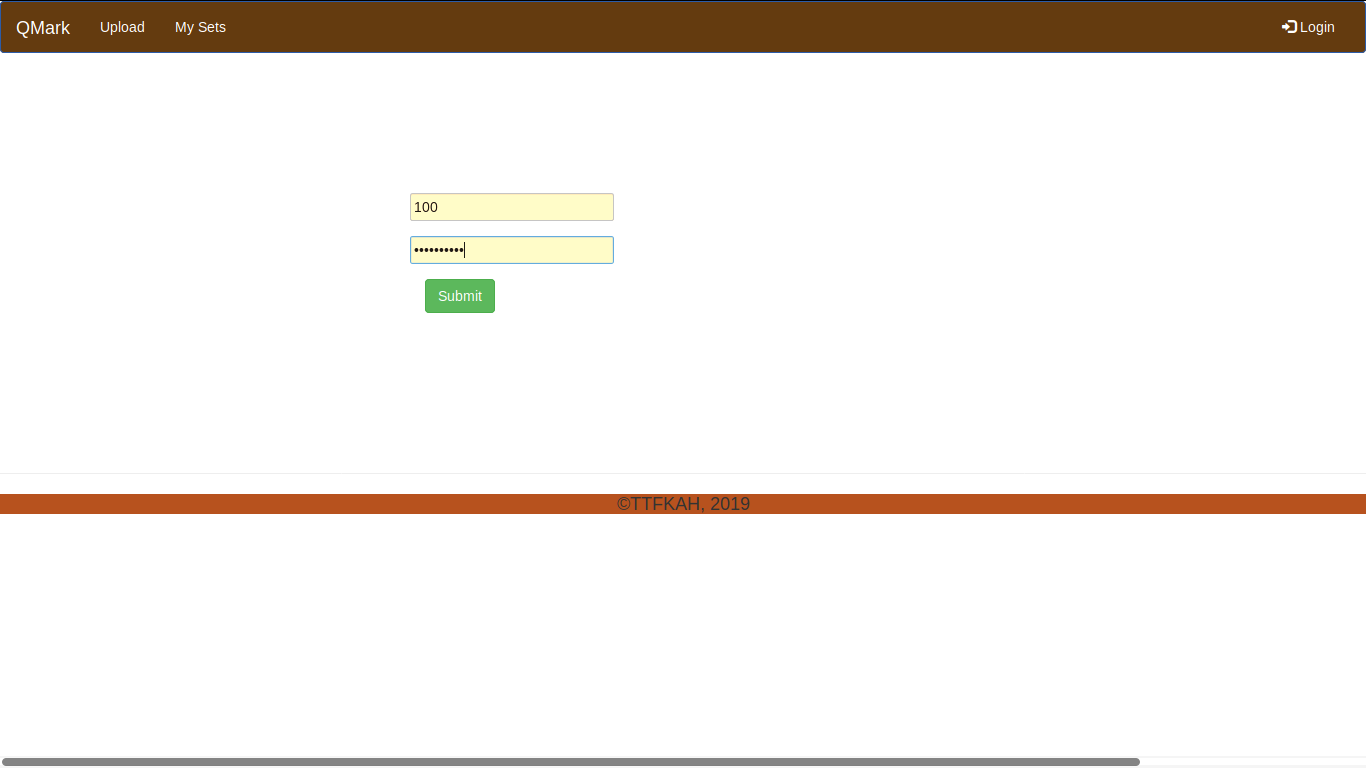
\includegraphics[width=\textwidth,height=\textheight,keepaspectratio]{4.png}
    
    \caption{Approximate Landing Page for Instructors of QMark on desktop}
    \label{fig:inst_loginpage}
\end{figure}

Figure \ref{fig:inst_loginpage} shows the login page that'll be used by the instructors to log into the QMark.



\begin{figure}[H]
    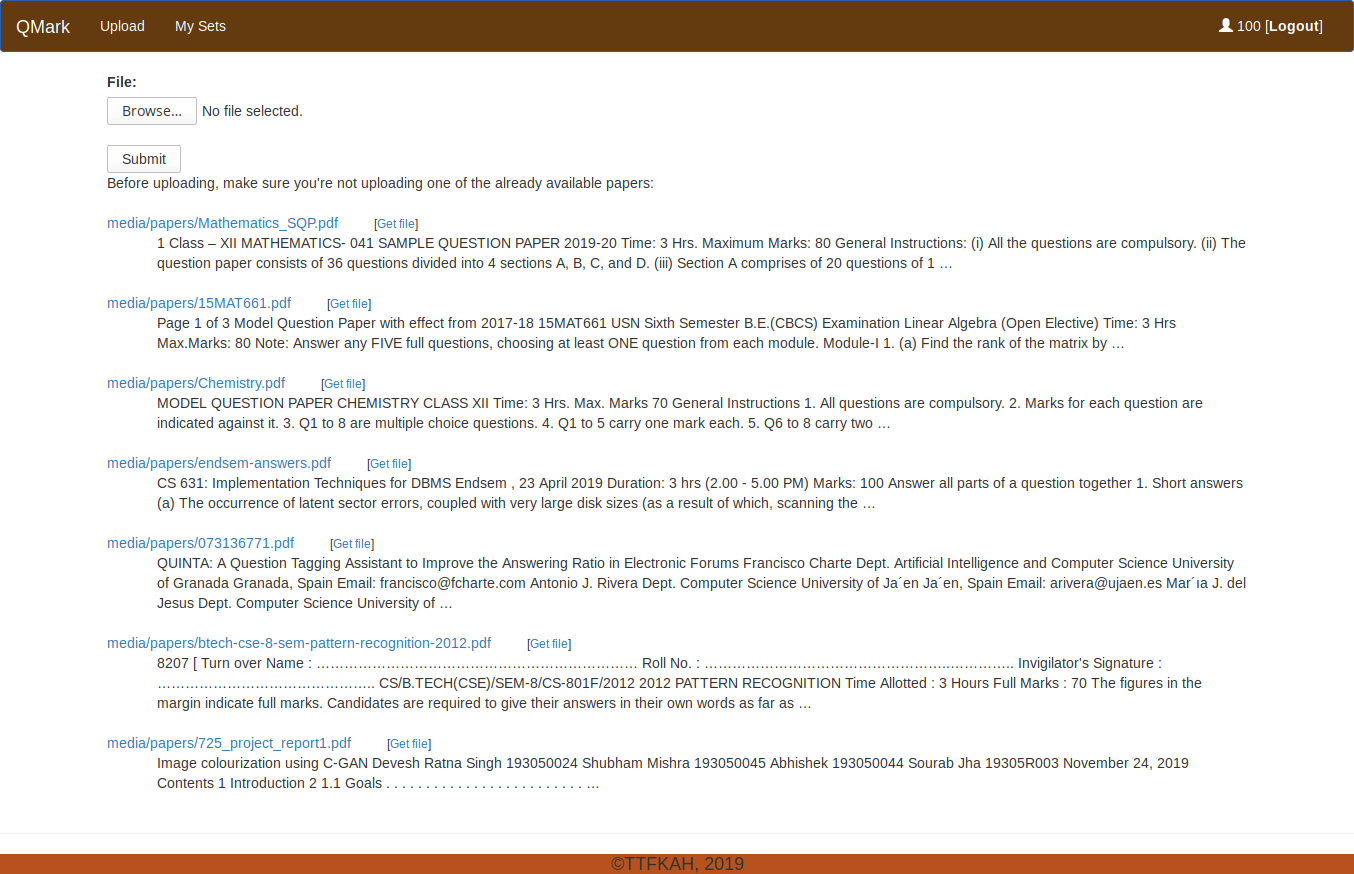
\includegraphics[width=\textwidth,height=\textheight,keepaspectratio]{5.png}
    \caption{Instructor's HomePage}
    \label{fig:inst_home}
\end{figure}
Figure \ref{fig:inst_home} shows the instructor's homepage which can be used to upload pdf files with questions from which questions will automatically be extracted.

\begin{figure}[H]
    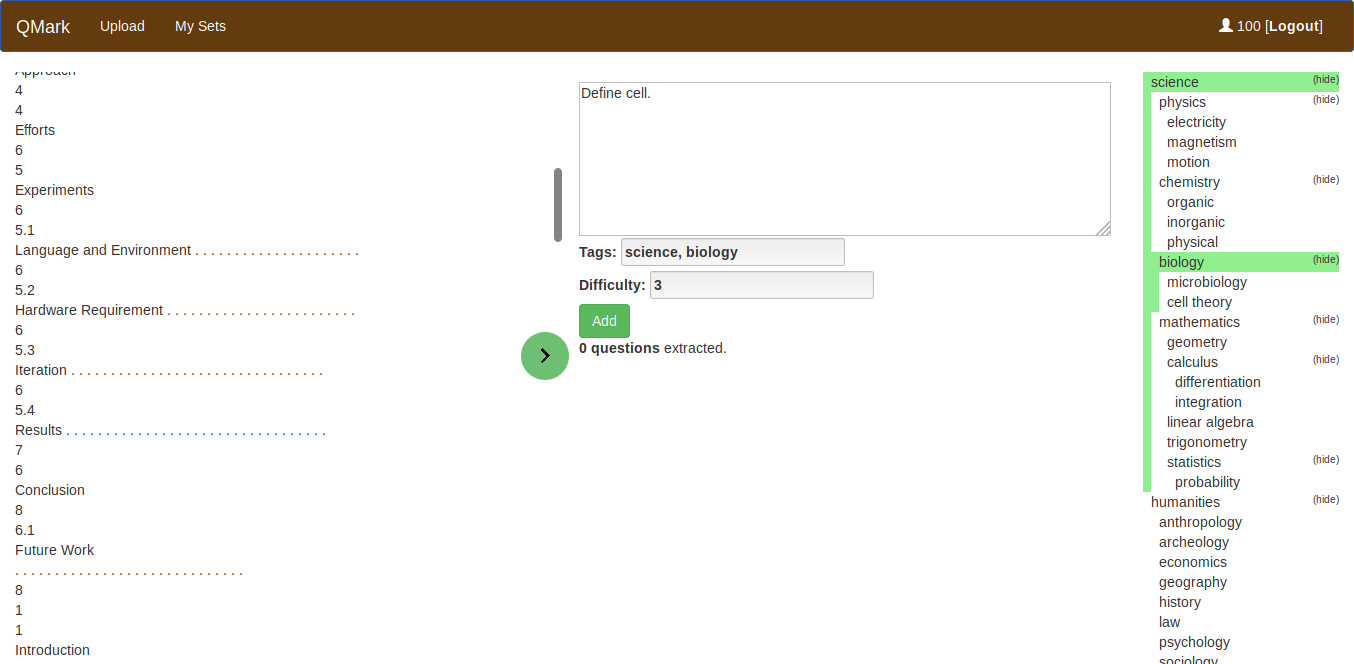
\includegraphics[width=\textwidth,height=\textheight,keepaspectratio]{6.png}
    \caption{Question Upload page}
    \label{fig:inst_upload}
\end{figure}
Once we select and upload a pdf file from Figure \ref{fig:inst_home}, we'll be redirected to the page in figure \ref{fig:inst_upload}. This page consists of three sections. The leftmost section has the extracted questions from the uploaded pdf file. The section in the middle will be used for adding questions to the Question Bank and the leftmost section is there for tagging questions.

\begin{figure}[H]
    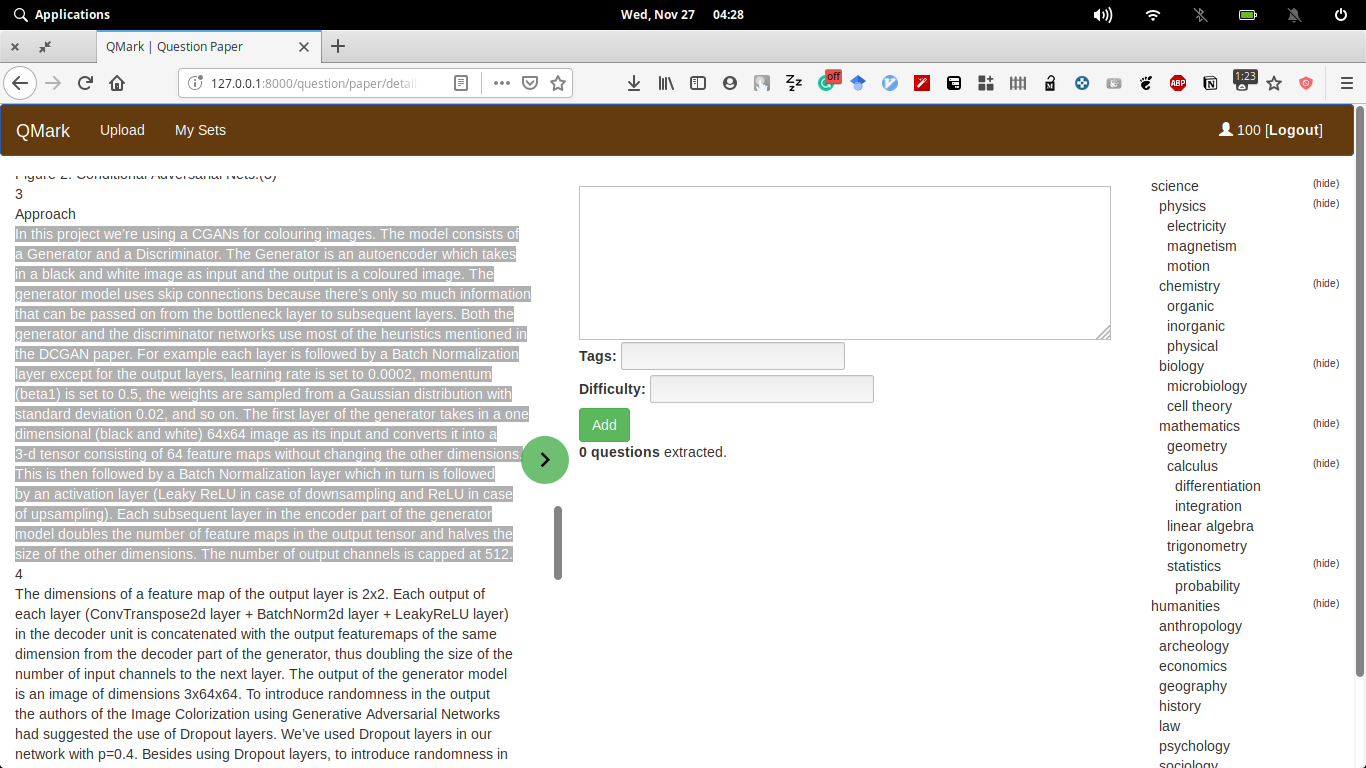
\includegraphics[width=\textwidth,height=\textheight,keepaspectratio]{7.png}
    \caption{QuestionPaper details page where questions can be added.}
    \label{fig:qp1}
\end{figure}

\begin{figure}[H]
    \includegraphics[width=\textwidth,height=\textheight,keepaspectratio]{{{8.0}}}
    
    \caption{Text selection to add as a question.}
    \label{fig:qp2}
\end{figure}
To select a particular question from the extracted questions, all we need to do is to select the question and click on the green arrow button. The question will automatically appear in the textbox as can be seen in figure \ref{fig:qp2}. Questions can also be entered manually by typing the question in the textbox.

\begin{figure}[H]
    \includegraphics[width=\textwidth,height=\textheight,keepaspectratio]{{{8.2}}}
    \caption{Selected tags while adding a question.}
    \label{fig:qp3}
\end{figure}
Questions can be tagged by putting the question in the text box and then selecting the appropriate tags, as shown in \ref{fig:qp3}. Since tags follow a strict hierarchy, if any tag is selected, all its ancestors are selected, too. Similarly, if any selected tag is unselected, all its descendants will be unselected, too.\par
Since most questions in a paper are mostly related, the tags used in the last question are saved and can be reused the next time this page is visited.\par
Also, difficulty can be added from the same form.

\begin{figure}[H]
    \includegraphics[width=\textwidth,height=\textheight,keepaspectratio]{{{8.3}}}
    \caption{Aspirant Landing Page}
    \label{fig:asp_landingpage}
\end{figure}
In the figure \ref{fig:asp_landingpage} we can see the landing page for aspirants. Clicking on the "Get Started" button at the bottom of the screen will redirect the aspirant to the login page (if not already logged in).

\begin{figure}[H]
    \includegraphics[width=\textwidth,height=\textheight,keepaspectratio]{{{9}}}
    \caption{Page for creating new question set.}
    \label{fig:asp_newqset}
\end{figure}
In figure \ref{fig:asp_newqset} we can see the page that can be used to create new question set once the aspirant has logged in. 


\begin{figure}[H]
    \includegraphics[width=\textwidth,height=\textheight,keepaspectratio]{{{10}}}
    
    \caption{A question paper with many questions parsed and added.}
    \label{fig:qp4}
\end{figure}

\begin{figure}[H]
    \includegraphics[width=\textwidth,height=\textheight,keepaspectratio]{{{11}}}
    \caption{Finding questions based on the tags selected. Tags highlighted in green are tags that are white-listed.}
    \label{fig:asp_qset1}
\end{figure}
Topics can be white-listed by clicking on the appropriate tag once. White-listing two topics shows us questions that have both the tags.

\begin{figure}[H]
    \includegraphics[width=\textwidth,height=\textheight,keepaspectratio]{{{12}}}
    \caption{Tags highlighted in pink are black-listed.}
    \label{fig:asp_qset2}
\end{figure}
Topics can be black-listed by clicking on the corresponding tag twice. Black-listed tags are highlighted in pink. Clicking on the selected tag for the third time causes the tag to be unselected.

\begin{figure}[H]
    \includegraphics[width=\textwidth,height=\textheight,keepaspectratio]{{{13}}}
    \caption{Black-listing and white-listing topics}
    \label{fig:asp_qset3}
\end{figure}

\begin{figure}[H]
    \includegraphics[width=\textwidth,height=\textheight,keepaspectratio]{{{14}}}
    \caption{Selecting a question from the set of questions.}
    \label{fig:asp_qset4}
\end{figure}
A question can be added to the question set by clicking on the "Add" button as can be seen from figure \ref{fig:asp_qset4}.

\begin{figure}[H]
    \includegraphics[width=\textwidth,height=\textheight,keepaspectratio]{{{15}}}
    \caption{List of question sets.}
    \label{fig:asp_qset5}
\end{figure}
Figure \ref{fig:asp_qset5} shows the list of question sets created by an aspirant. The question set can be visited by clicking on the "Public link" link.

\begin{figure}[H]
    \includegraphics[width=\textwidth,height=\textheight,keepaspectratio]{{{16}}}
    \caption{Question Set}
    \label{fig:asp_qset6}
\end{figure}

\section{Future Work}
This project can be used by instructors to add questions to a question bank. The question bank will contain tagged questions. Aspirants will be able to select questions from here based on white-listed and black-listed topics. The user interface is pretty intuitive and easy to use. Future work includes:
\begin{itemize}
    \item developing APIs that can be used to integrate QBank with Moodle and SAFE App.
    \item adding Machine Learning Algorithms, once we have enough questions in our tagged questions database, that can be used to suggest possible tags for a question.
\end{itemize}
\end{document}
